\documentclass[12pt,a4paper]{report}
\usepackage[utf8]{inputenc}
\usepackage[T1]{fontenc}
\usepackage[french]{babel}
\usepackage{graphicx}
\usepackage{geometry}
\usepackage{setspace}
\usepackage{hyperref}
\usepackage{titlesec}
\usepackage{xcolor}
\geometry{margin=2.5cm}
\usepackage{array}   % Pour personnaliser les colonnes
\usepackage[none]{hyphenat} % dans le préambule
\usepackage{float}
\usepackage{makecell}


\onehalfspacing

\titleformat{\chapter}[display]
{\normalfont\bfseries\huge}{\chaptername\ \thechapter}{20pt}{\Huge}
\titleformat{\section}
{\normalfont\Large\bfseries}{\thesection}{1em}{}

\begin{document}
	
	\tableofcontents
	
	\chapter{Contexte du Projet}
	
	\section{Projet de Fin d’Études}
	
	Dans le cadre de notre formation en Génie Informatique à l’École des Hautes Études d’Ingénierie d’Oujda (EHEIO), nous devons réaliser un Projet de Fin d’Études (PFE), visant à consolider et approfondir les compétences acquises durant notre parcours. Ce stage représente une étape cruciale, permettant de transposer les connaissances théoriques dans un environnement professionnel concret.
	
	L’objectif principal est de se familiariser avec les réalités du marché du travail, particulièrement dans le domaine de l’informatique, en perpétuelle évolution. Ce projet offre ainsi l’opportunité d’appliquer nos acquis académiques à des problématiques réelles, tout en développant une approche pratique et méthodique de la gestion de projets technologiques.
	
	Ce stage s’est déroulé dans une entreprise adoptant une méthodologie Scrum, l’une des approches Agile les plus répandues dans le secteur informatique. Cette immersion professionnelle a été l’occasion découvrir le fonctionnement d’une équipe projet en conditions réelles, d'appliquer les principes Agile (itérations, sprints, réunions quotidiennes) dans un cadre professionnel, et de collaborer avec des experts et assimiler les bonnes pratiques en gestion de projets logiciels.
	
	L’utilisation de Scrum a renforcé ma compréhension des processus modernes de développement, tout en améliorant mes capacités d’adaptation et de travail en équipe. Cette expérience a été déterminante pour affiner ma vision du métier d’ingénieur informatique et préparer mon intégration dans le monde professionnel.
	
	Dans ce chapitre, nous commencerons par présenter l’entreprise d’accueil, avant de procéder à une description détaillée des besoins du projet. Cette description comprendra l’identification du problème posé, l’analyse des besoins fonctionnels et non fonctionnels, ainsi que les solutions envisagées pour y répondre.
	
	\section{Entreprise d’accueil}
	
	Ce stage a été réalisé au sein de l’entreprise Algolus, située à Oujda, spécialisée dans les solutions innovantes en intelligence artificielle. Démarré le 24 février 2024, il m’a permis de m’immerger dans un environnement professionnel exigeant, où j’ai pu collaborer avec des experts en IA et en ingénierie logicielle.
	
	\begin{figure}[H]
		\centering
		
\includegraphics[width=0.3\textwidth]{algolus-logo.png}
		\caption{\textit{Logo de Algolus}}
		\label{fig:algolus-logo}
	\end{figure}
	
	\subsection{Description de l’entreprise}
	
	Algolus est une agence web marocaine, créée en 2020, spécialisée dans la conception et le développement de solutions informatiques adaptées aux besoins des clients. Elle s'engage à offrir à ses clients une communication en ligne efficace et sur mesure.

	Ses prestations incluent :
	
	\renewcommand{\labelitemi}{$\bullet$}
	\begin{itemize}
		\item Création et gestion de sites web (dynamiques, statiques, e-commerce, CMS)
		\item Développement d'applications web (mode hybride)
		\item Stratégie digitale complète : infographie, publicité en ligne, marketing digital, community management, E-réputation.
	\end{itemize}
	
	\subsection{Fiche technique de l'entreprise}
	
	Le tableau 1.1 récapitule la fiche technique de l'entreprise Algolus :
	
	\begin{table}[htbp]
		\centering
		\caption{\textit{Fiche technique de l'entreprise Algolus}}
		\begin{tabular}{|l|l|}
			\hline
			\textbf{Dénomination sociale} & Algolus \\
			\hline
			\textbf{Date de création} & 07/10/2020 \\
			\hline
			\textbf{Forme juridique} & SARL \\
			\hline
			\textbf{Capital} & 100.000 Dh \\
			\hline
			\textbf{Chiffre d'affaires} & Indisponible \\
			\hline
			\textbf{Activités} & Développement informatique et marketing digital \\
			\hline
			\textbf{Effectif} & 10 \\
			\hline
			\textbf{Dirigeant} & Radwane BERAHIOUI \\
			\hline
			\textbf{Coordonnées} & \makecell[l]{+212 6644 35967 \\ Redwan.Berahioui@algolus.ma \\ www.algolus.ma \\ IMMEUBLE OUASSIM, Bd Mohammed VI, Oujda 60000} \\
			\hline
		\end{tabular}
		\label{tab:fiche-technique-algolus}  % Pour référence avec \ref
	\end{table}
	
	\subsection{Organigramme de l’entreprise}
	
	La figure 1.2 présente l'organigramme de l'entreprise Algolus :
	
	\begin{figure}[H]
		\centering
		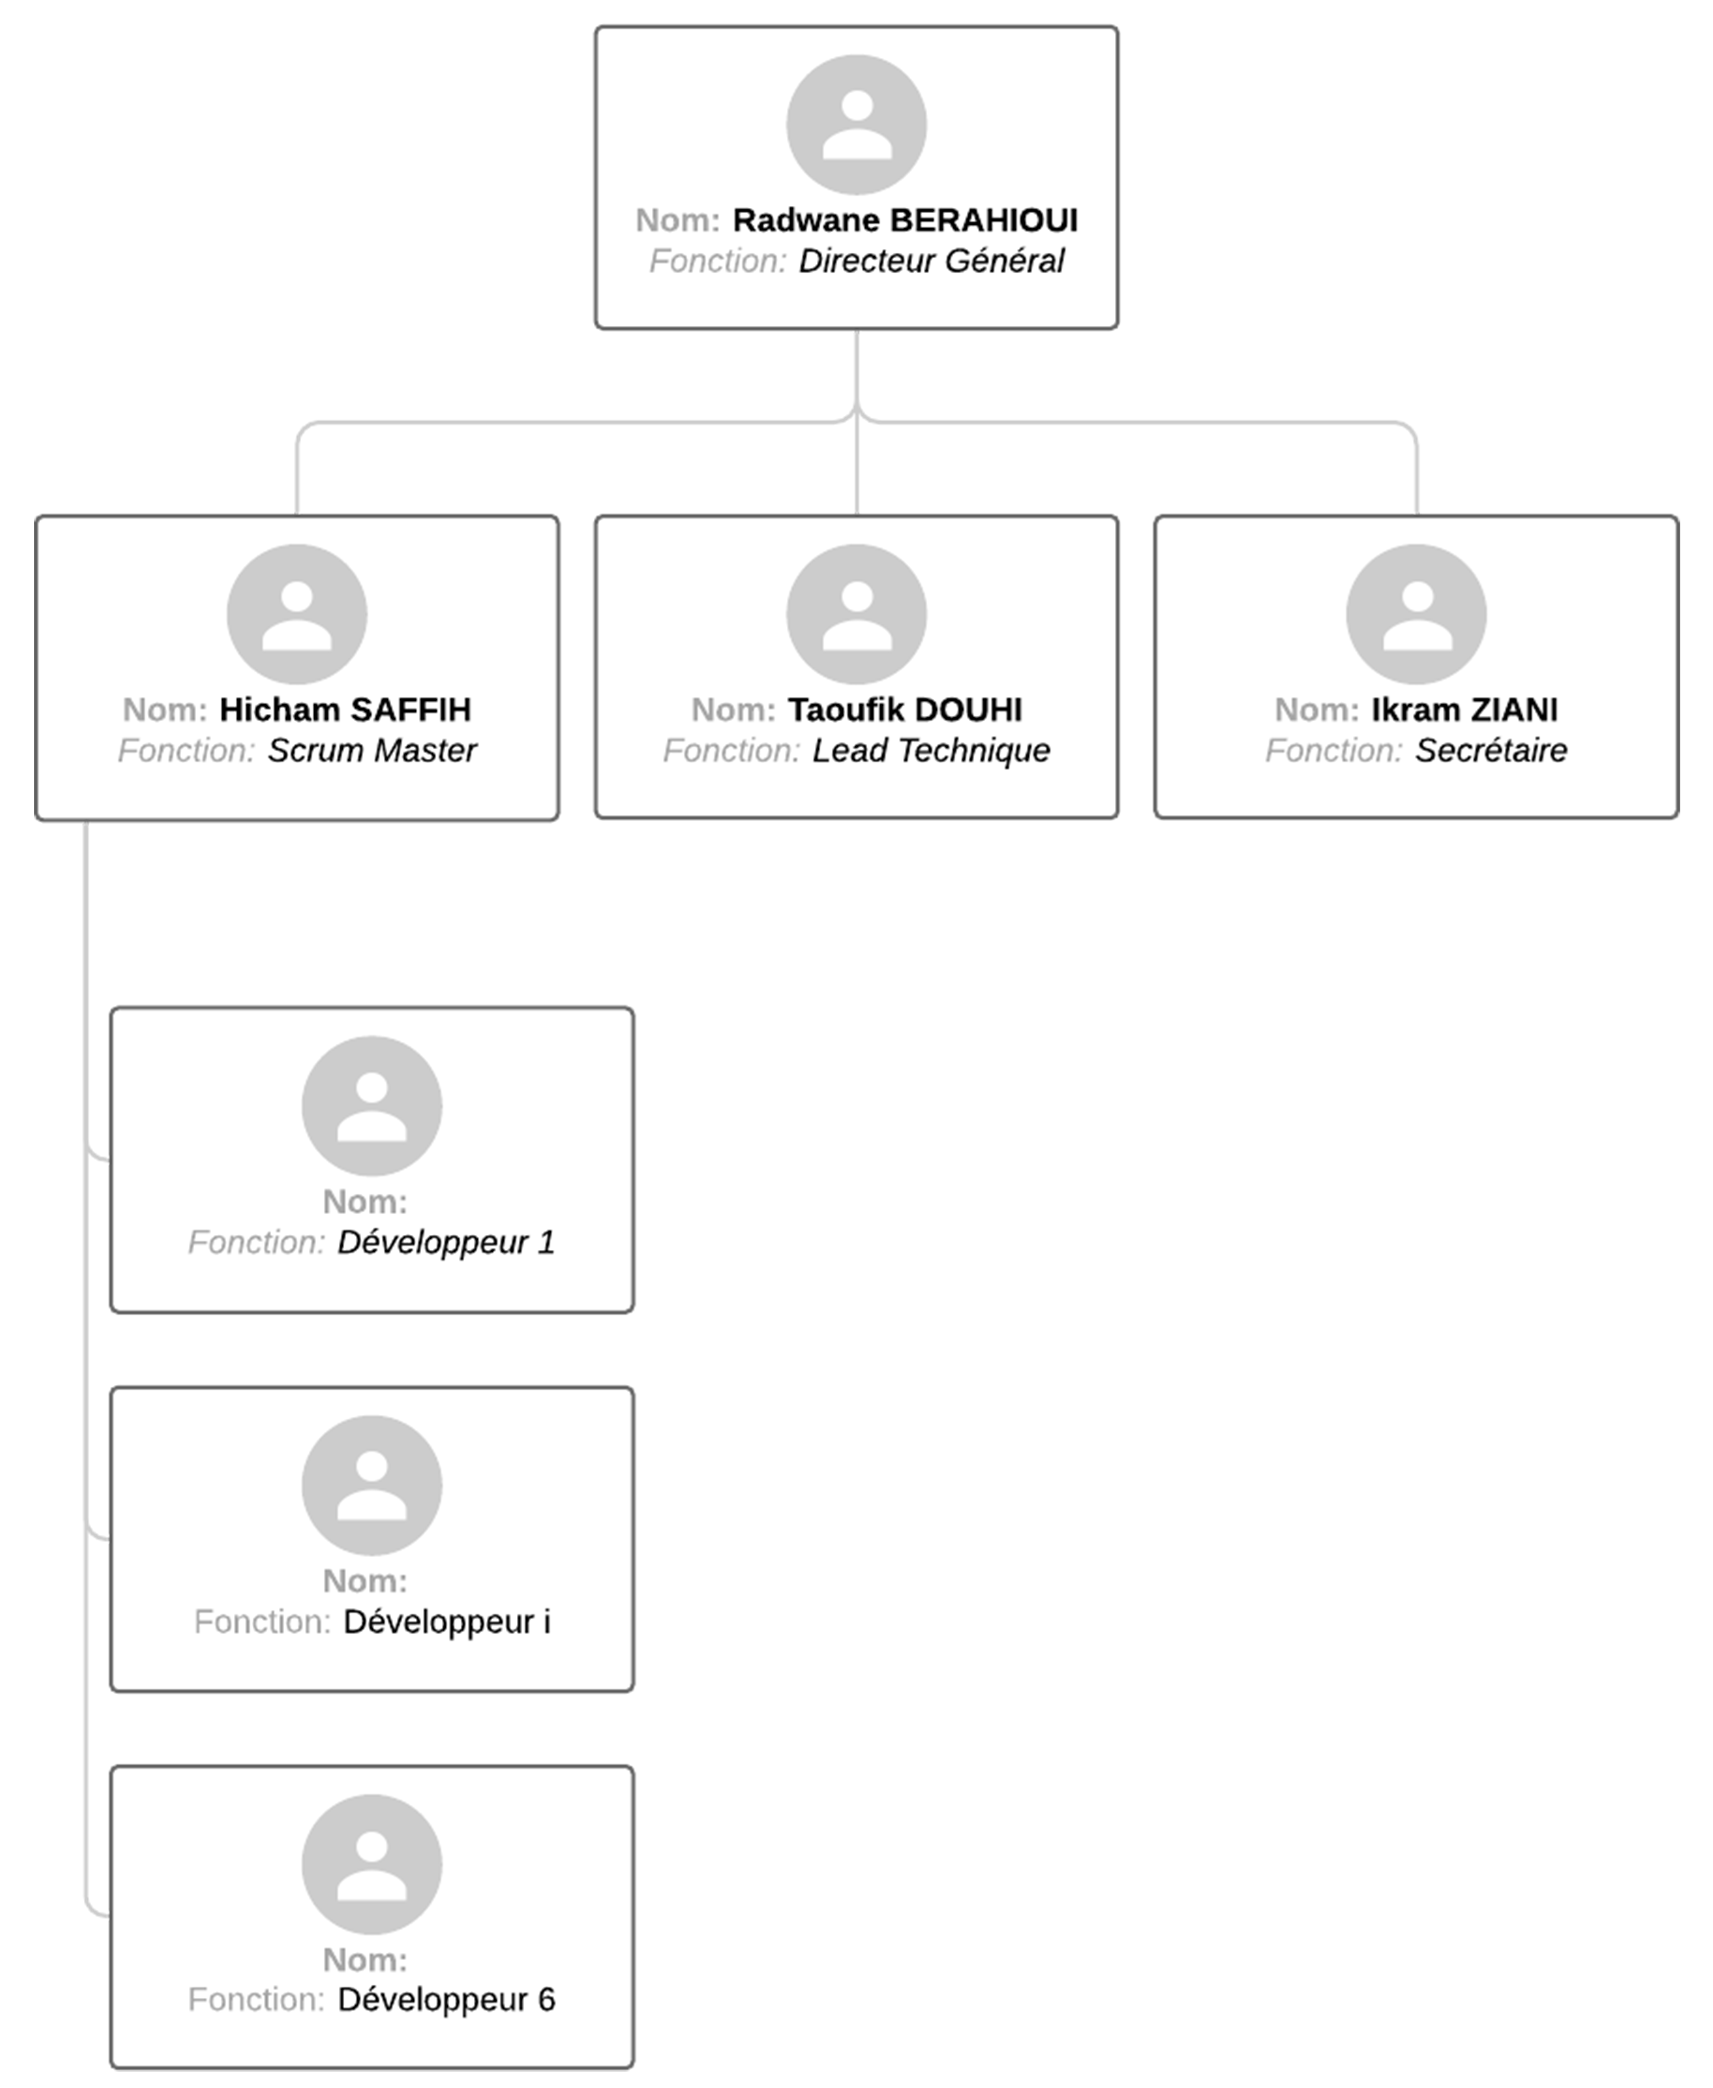
\includegraphics[width=1\textwidth]{algolus-organigramme.png}
		\caption{\textit{Organigramme de l'entreprise Algolus}}
		\label{fig:algolus-organigramme}
	\end{figure}
	
	\section{Description des besoins}
	
	\subsection{Problème}
	
	Dans le développement logiciel, la détection et la correction des erreurs représentent un défi majeur, notamment en raison de la diversité des sources d’anomalies (logs, stack traces, captures d’écran, retours utilisateurs, etc.) et de la complexité croissante des applications. Les méthodes traditionnelles de débogage reposent souvent sur une analyse manuelle, ce qui est chronophage et sujet à des erreurs humaines. De plus, les solutions existantes peinent à offrir une approche générique et intelligente pour interpréter ces anomalies et proposer des correctifs pertinents.
	
	Ce défi prend une dimension particulière dans le cadre des activités de Algolus. La complexité des systèmes gérés par l'entreprise, caractérisés par des architectures microservices distribuées, des intégrations multiples avec des partenaires externes et des exigences strictes de conformité, amplifie les difficultés de diagnostic des anomalies. Les équipes techniques consacrent actuellement un volume considérable de leurs ressources temporelles à l'analyse manuelle des incidents, retardant d'autant les mises en production. Par ailleurs, la variété des clients et des cas d'usage entraîne une hétérogénéité des remontées d'erreurs (rapports techniques détaillés pour les clients corporate vs. simples captures d'écran pour les utilisateurs finaux), ce qui rend inefficaces les outils de monitoring conventionnels utilisés jusqu'à présent. Ce constat a motivé l'entreprise à explorer des solutions d'IA générative capables d'unifier l'interprétation des anomalies.
	
	\subsection{Les besoins fonctionnels}
	
	Les besoins fonctionnels définissent les actions spécifiques que le système doit accomplir pour répondre aux exigences métier. Ils décrivent "quoi" le logiciel doit faire, sous la forme de fonctionnalités concrètes, de processus et d'interactions avec l'utilisateur. Ces exigences sont formulées par les parties prenantes : clients, utilisateurs, et équipe produit,  et servent de base à la conception des cas d’usage et des scénarios de test.
	
	Les besoins fonctionnels suivants ont été identifiés pour garantir que le système de diagnostic d’erreurs réponde efficacement aux attentes des utilisateurs et des équipes techniques :
	
	\begin{enumerate}
		
		\item \textbf{Collecte et Pré-traitement des Données} : Extraction automatique des erreurs et des anomalies des systèmes à partir de :
		stacktraces, parsing des logs, captures d’écran, retours utilisateurs.
		
		\item \textbf{Analyse et Compréhension} : Analyse sémantique de retours d’erreurs, enrichissement contextuel : requêtage d’une base de connaissances (documentation technique, correctifs historiques) via RAG (Retrieval-Augmented Generation).
		
		\item \textbf{Génération de Solutions} : Explication en langage naturel des causes racines, génération de correctifs (ex: snippets de code, étapes de résolution).
		
		\item \textbf{Interfaces utilisateurs} : Soumission des erreurs via des formulaires web pour uploader des stacktraces et des captures d'écran, visualisation des résultats : Dashboard interactif (erreurs en cours, historiques, statistiques).

	\end{enumerate}
	
	\subsection{Les besoins non fonctionnels}
	
	Les besoins non fonctionnels caractérisent "comment" le système doit fonctionner, en précisant ses contraintes de qualité, de performance et d’infrastructure. Contrairement aux besoins fonctionnels, ils ne décrivent pas des fonctionnalités mais des critères tels que la rapidité, la sécurité, la scalabilité ou la facilité de maintenance. Leur respect est essentiel pour assurer la robustesse et l’efficacité du système en conditions réelles.
	
	Pour garantir une intégration harmonieuse dans l’écosystème existant et une expérience utilisateur optimale, les besoins non fonctionnels suivants ont été définies :
	
	\begin{enumerate}
		
		\item \textbf{Performances} : Temps de réponse optimisé, et scalabilité : Support de plusieurs requêtes simultanées.
		
		\item \textbf{Intégration et Interopérabilité} : API REST : Endpoints standardisés et format de réponse avec schéma cohérent, support offline : fonctionnement local avec Ollama.
		
		\item \textbf{Sécurité et Confidentialité} : Protection des données par chiffrement des échanges et anonymisation des logs utilisateurs (RGPD), et authentification : JWT pour l’accès aux APIs sensibles.	
		
		\item \textbf{Expérience Utilisateur} : Ergonomie : interface intuitive, Dark/Light mode et thèmes accessibles.

		
	\end{enumerate}
	
	\subsection{Solutions envisagées}
	
	Ce projet vise à développer une application intelligente et modulaire permettant de détecter et de corriger automatiquement les anomalies logicielles. Les objectifs spécifiques incluent :
	
	\renewcommand{\labelitemi}{$\bullet$}
	\begin{itemize}
		\item Détecter avec un taux de réussite d'au moins 80\% les anomalies logicielles sur des sources multimodales.
		
		\item Proposer des correctifs pertinents dans plus de 70\% des cas.
		
		\item Optimiser le temps moyen de résolution d’erreurs de 30\% par rapport aux méthodes manuelles.
	\end{itemize}
	
	
	
	Pour atteindre ces objectifs, le projet s’appuie sur une architecture innovante :
	
	\begin{enumerate}
		\item \textbf{Analyse Multimodale des Erreurs} : Implémenter un système capable d’interpréter des données hétérogènes (stack traces, logs texte, captures d’écran, etc.), et utiliser des techniques de RAG pour enrichir les requêtes avec une base de connaissances (documentation technique, résolutions d’erreurs courantes).
		
		\item \textbf{Génération Automatique de Correctifs} : Exploiter des LLMs (via Ollama) pour suggérer des corrections précises et contextualisées.
		
		\item \textbf{Intégration et Scalabilité} : Développer un backend Spring Boot flexible, couplé à LangChain4J pour orchestrer les appels IA, et un système de gestion de base de données qui prend en charge les bases de données vectorielles, comme PostgeSQL, et permettre une extension future via des connecteurs pour différents outils de monitoring.
		
		\item \textbf{Optimisation et Évaluation} : mesurer l’efficacité du système via des métriques de précision (taux de détection, pertinence des correctifs), et effectuer un Benchmark : comparaison sur des jeux de données communs.
		
	\end{enumerate}
	

	
	\chapter{Analyse et modélisation}
	
	\section{Importance de l'analyse}
	
	L’analyse constitue une étape clé dans tout projet de développement informatique, car elle permet de bien comprendre les besoins du client et les contraintes du système à réaliser. Elle sert à identifier les fonctionnalités attendues, à détecter les éventuelles incohérences et à poser les bases d’une conception solide. Une analyse bien menée réduit considérablement les risques d’erreurs en phase de développement, facilite la planification du travail et améliore la qualité globale du produit final. Elle est donc essentielle pour assurer la réussite du projet.
	
	Dans ce chapitre, nous présentons une introduction à la modélisation UML en rappelant ses principes fondamentaux et son utilité dans le développement logiciel. Par la suite, nous exposerons les différents types de diagrammes utilisés dans notre étude, à savoir : le diagramme de cas d’utilisation, les diagrammes de séquence, ainsi que le diagramme de classes.
	
	\section{Unified Modeling Language}
	
	Dans le cadre d’un projet de développement informatique, la modélisation UML (Unified Modeling Language) joue un rôle essentiel en facilitant la compréhension, la conception et la communication autour du système à développer. UML propose un ensemble normalisé de diagrammes qui permettent de représenter visuellement les différentes dimensions d’un logiciel, telles que la structure, le comportement et les interactions entre les composants.
	
	L’utilisation de diagrammes UML, comme les diagrammes de cas d’utilisation, de classes ou de séquence, permet de clarifier les besoins fonctionnels et non fonctionnels dès les premières phases du projet, de favoriser une meilleure communication entre les développeurs, les analystes et les clients, de détecter plus tôt les incohérences ou erreurs potentielles dans la conception, et aussi de servir de documentation technique structurée pour le développement, les tests et la maintenance future du logiciel.
	
	Ainsi, UML constitue un outil précieux pour assurer la qualité, la cohérence et la pérennité d’un projet informatique, en apportant une vision globale et partagée du système.
	
	\section{Diagramme de cas d'utilisation}
	
	\subsection{Définition}
	
	Un diagramme de cas d'utilisation est une représentation visuelle des interactions entre les acteurs (utilisateurs, systèmes) et les fonctionnalités d'une application. Il identifie les besoins métiers sous forme d'actions (cas d’utilisation) et montre qui fait quoi, sans entrer dans les détails techniques.
	
	\subsection{Acteurs}
	
	Dans un diagramme de cas d'utilisation, les acteurs sont les entités qui interagissent avec le système pour accomplir un objectif précis. Un acteur peut être primaire (s'il est déclencheur d'un cas d'utilisation) ou secondaire (intervient dans un cas d'utilisation mais ne le déclenche pas). D'une autre part, un acteur peut être humain ou bien un acteur système.
	
	Trois types d'acteurs sont impliqués dans notre cas :
	
	\begin{itemize}
		\item \textbf{Utilisateur} : peut être un développeur ou un testeur qui rapporte une erreur, et peut interagir via une API REST ou bien une interface web.
		
		\item \textbf{Administrateur du système} : responsable de la mise à jour des connaissances du système et de la configuration des modèles.
		
		\item \textbf{Système} : le moteur de traitement intelligent, responsable d'analyser les anomalies, et de proposer des correctifs appropriés.
	\end{itemize}
	
	\subsection{Diagramme de cas d'utilisation}
	
	La figure 2.1 présente le diagramme de cas d'utilisation de notre application :
	
	\begin{figure}[H]
		\centering
		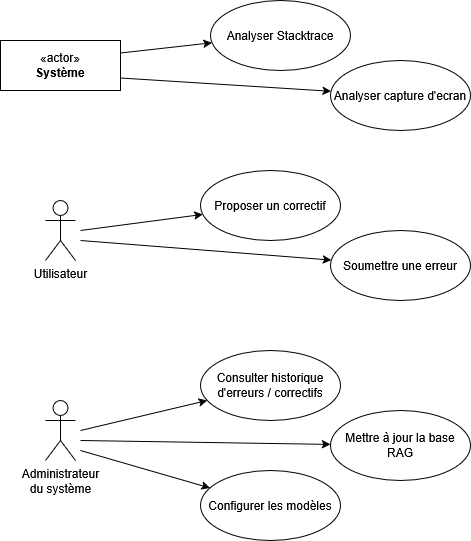
\includegraphics{use-case.drawio.png}
		\caption{\textit{Diagramme de cas d'utilisation}}
		\label{fig:use-case}
	\end{figure}
	
	\section{Diagrammes de séquences}
	
	\subsection{Définition}
	
	Un diagramme de séquences est un type de diagramme UML, utilisé pour modéliser les interactions entre les différents objets ou composants d'un système dans un scénario précis. Il met en évidence l'ordre chronologique des messages échangés entre les acteurs et les objets, les interactions dynamiques entre les éléments du système, et la durée de vie des objets participant au scénario.
	
	\subsection{Diagramme de séquences principal}
	
	Cette application d'analyse d'erreurs techniques repose sur une architecture modulaire, où chaque composant joue un rôle précis dans le traitement des requêtes. Voici une présentation des éléments clés qui permettent au système de comprendre, contextualiser et répondre aux problèmes soumis par les utilisateurs :
	
	\begin{itemize}
		
		\item \textbf{Utilisateur} : L'Utilisateur constitue le point de départ du système. Ce composant représente l'acteur humain qui interagit avec l'application via une interface web ou des appels API. Il soumet des requêtes contenant des stacktraces d'erreur et éventuellement des captures d'écran.
		
		\item \textbf{Agent AI} : sert de chef d'orchestre principal dans l'architecture. Ce service intelligent coordonne l'ensemble du processus d'analyse. Il reçoit les requêtes brutes de l'utilisateur, les enrichit en combinant plusieurs techniques avancées comme le RAG et la mémoire conversationnelle, puis les présente au modèle de langage sous une forme optimale.
		
		\item \textbf{ChatModel} : incarne le moteur de génération de langage naturel. Ce composant spécifique, configuré pour utiliser des modèles locaux ou externes, transforme les prompts structurés en analyses techniques détaillées.
		
		\item \textbf{RAG (Retrieval-Augmented Generation)} : apporte une dimension documentaire aux analyses. Composé de trois éléments principaux - un modèle d'embedding, un stockage vectoriel et un moteur de recherche - ce pipeline sophistiqué permet d'enrichir les réponses du LLM avec des connaissances provenant d'une base documentaire technique. Le processus transforme d'abord les requêtes et documents en vecteurs, puis effectue des recherches de similarité dans le stockage vectoriel avant d'injecter les documents pertinents dans le contexte du LLM.
		
		\item \textbf{LLM (Large Language Model)} : représente le cœur cognitif du système. Ce modèle linguistique à grande échelle possède une compréhension approfondie du langage naturel et des concepts techniques. Capable de traiter des stacktraces complexes et d'identifier des patterns d'erreur, il génère des analyses structurées qui incluent généralement la classification de l'erreur, sa cause probable, et des solutions potentielles. Son fonctionnement est optimisé par le contexte fourni par la mémoire conversationnelle et les documents retrouvés via le RAG.
		
		\item \textbf{ChatMemory} : joue un rôle crucial dans la maintien du contexte conversationnel. Implémentée comme une mémoire à fenêtre glissante, elle conserve les N dernières interactions de chaque session utilisateur, identifiée par un MemoryId unique. Cette mémoire permet au LLM de maintenir une cohérence dans les échanges et de se souvenir des points clés abordés précédemment dans la conversation, essentiel pour les analyses techniques itératives où l'utilisateur affine progressivement sa requête.
		
	\end{itemize}
	
	Le diagramme de séquences dans la figure 2.2 décrit le flux de messages entre ces composants.
	
	\begin{figure}[H]
		\centering
		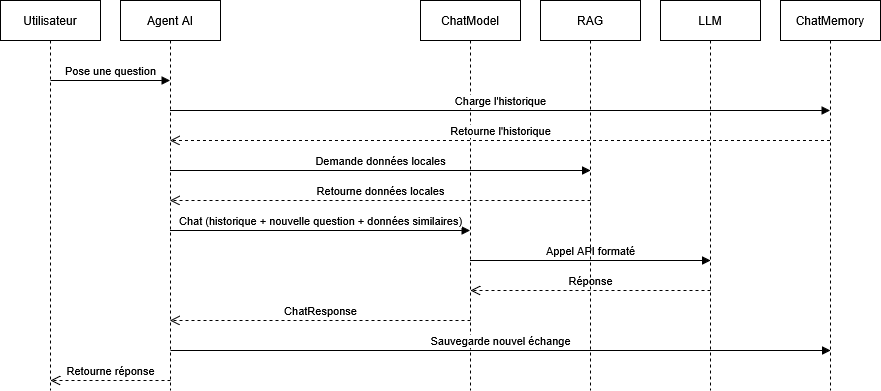
\includegraphics[width=\textwidth]{ds-ai-agent.drawio.png}
		\caption{\textit{Diagramme de séquences décrivant le fonctionnement d'un agent AI}}
		\label{fig:ds-ai-agent.drawio}
	\end{figure}
	
	\subsection{Diagramme de séquences spécifique : RAG}
	
	Nous allons creuser un peu dans les composants du système RAG, voici une énumération de ces composants avec chacun son rôle :
	
	\begin{itemize}
		
		\item \textbf{Resource} : Constitue la matière première du système RAG. Il s'agit de la source originelle des données qui alimenteront la base de connaissances. Ces ressources peuvent prendre diverses formes : fichiers PDF contenant de la documentation technique, pages web de référence, extraits de bases de données, ou tout autre support contenant des informations pertinentes. Le système doit être capable de traiter ces ressources hétérogènes, qu'elles proviennent de systèmes internes ou de sources externes. La qualité et l'actualité des resources déterminent en grande partie l'efficacité finale du système RAG.
		
		\item \textbf{Tokenizer} : Joue un rôle fondamental dans le prétraitement du texte. Ce composant décompose le contenu textuel en unités significatives appelées tokens, qui peuvent correspondre à des mots entiers, des sous-mots ou même des caractères individuels selon la méthode employée. Des algorithmes avancés comme ceux proposés par HuggingFace permettent une tokenisation optimale qui préserve le sens tout en gérant les particularités linguistiques. La tokenisation est cruciale car elle influence directement la qualité des embeddings générés ultérieurement.
		
		\item \textbf{DocumentParser} : Assure la transformation des ressources brutes en documents structurés. Ce composant doit comprendre divers formats de fichiers (PDF, HTML, Markdown, etc.) et en extraire le contenu textuel significatif tout en conservant les métadonnées importantes. Des bibliothèques spécialisées comme sont souvent employées pour cette tâche complexe. Le DocumentParser nettoie également le texte en supprimant les éléments non pertinents (en-têtes, pieds de page, balises HTML) pour ne conserver que l'information essentielle.
		
		\item \textbf{Document} : Représente la forme normalisée et standardisée des informations après traitement. Chaque document contient non seulement le texte brut nettoyé, mais aussi des métadonnées descriptives (titre, auteur, date de création, source) qui faciliteront son identification et son utilisation ultérieure. Un identifiant unique est attribué à chaque document pour permettre son suivi tout au long du pipeline. Cette structuration rigoureuse est essentielle pour maintenir la cohérence des données dans les étapes suivantes du processus RAG.
		
		\item \textbf{EmbeddingModel} : Est au cœur de la transformation sémantique du système. Ce modèle sophistiqué convertit le texte en représentations vectorielles denses (embeddings) qui capturent le sens profond des contenus. Des modèles sont spécialisés dans cette tâche produisent des vecteurs où la similarité spatiale correspond à la similarité sémantique. La qualité de l'EmbeddingModel détermine directement la capacité du système à retrouver des documents pertinents pour une requête donnée.
		
		\item \textbf{EmbeddingStoreIngestor} : Orchestre le processus complet d'indexation des documents. Ce composant supervise plusieurs opérations critiques : il applique la tokenisation et la segmentation des textes, déclenche la génération des embeddings via l'EmbeddingModel, et gère le stockage final dans l'EmbeddingStore. L'EmbeddingStoreIngestor implémente souvent des stratégies de traitement par lots pour optimiser les performances et peut gérer des pipelines complexes de prétraitement avant la vectorisation.
		
		\item \textbf{EmbeddingStore} : Sert de mémoire à long terme au système RAG. Cette base de données vectorielle spécialisée stocke les embeddings générés et permet des recherches rapides de similarité. L'EmbeddingStore doit supporter des opérations massives d'insertion tout en maintenant des temps de réponse faibles pour les requêtes.
		
		\item \textbf{Retriever} : Est le composant qui établit le pont entre les questions des utilisateurs et la base de connaissances. Lors d'une requête, le Retriever transforme d'abord la question en embedding, puis recherche dans l'EmbeddingStore les documents dont les vecteurs sont les plus proches. Ce composant implémente des algorithmes de similarité vectorielle (cosine similarity par exemple) et peut être finement paramétré (nombre de résultats retournés, seuil de similarité minimal). Le Retriever joue ainsi un rôle déterminant dans la pertinence des résultats fournis au LLM.
		
	\end{itemize}
	
	Le diagramme de séquences dans la figure 2.3 résume ce processus.
	
	\begin{figure}[H]
		\centering
		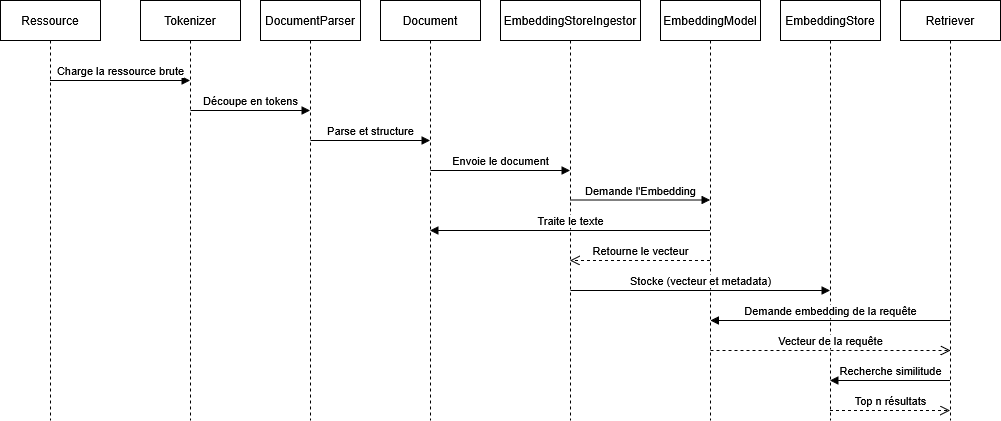
\includegraphics[width=\textwidth]{ds-rag.drawio.png}
		\caption{\textit{Diagramme de séquences décrivant le fonctionnement d'un RAG}}
		\label{fig:ds-rag.drawio}
	\end{figure}
	
	\chapter{Réalisation}
	
	Ce chapitre présente la phase de concrétisation du projet, où les choix techniques et architecturaux se traduisent en une implémentation fonctionnelle. Il décrit l'environnement de développement (outils, frameworks, librairies, etc.), l'architecture logicielle retenue et son adéquation avec les besoins, les défis techniques rencontrés et les solutions apportées, et les composants clés implémentés avec des extraits de code significatifs, et des captures d'écran illustrant les résultats obtenus.

	\section{Stack technique}
	
	\subsection{Langages}
	
	\subsubsection{Java}
	
	\begin{figure}[H]
		\begin{minipage}{0.8\textwidth}
			Java est un langage de programmation orienté objet, robuste et multiplateforme, largement utilisé dans le développement d'applications d'entreprise. Sa forte typographie, sa gestion automatique de la mémoire (via le garbage collector) et son écosystème riche (bibliothèques, frameworks) en font un choix idéal pour les systèmes backend complexes.
		\end{minipage}
		\hfill
		\begin{minipage}{0.15\textwidth}
			\begin{figure}[H]
				\centering
				
\includegraphics[width=\linewidth]{java-logo.png}
				\label{fig:java-logo}
			\end{figure}			
		\end{minipage}
	\end{figure}
		
	\subsection{Frameworks}
	
	\subsubsection{Spring}
	
	\begin{figure}[H]
		\begin{minipage}{0.8\textwidth}
			Spring est un framework modulaire pour Java, simplifiant le développement d'applications grâce à l’inversion de contrôle (IoC) et la programmation orientée aspect (AOP).
		\end{minipage}
		\hfill
		\begin{minipage}{0.15\textwidth} 
			\begin{figure}[H]
				\centering
				
\includegraphics[width=\linewidth]{spring-logo.png}
				\label{fig:spring-logo}
			\end{figure}
		\end{minipage}
	\end{figure}
	
	\subsubsection{Spring Boot}
	
	\begin{figure}[H]
		\begin{minipage}{0.8\textwidth}
			Spring Boot étend Spring en fournissant des configurations automatiques, un serveur embarqué (Tomcat, Netty) et des outils clés en main (Spring Data, Spring Security), permettant de créer des applications standalone rapidement.
		\end{minipage}
		\hfill
		\begin{minipage}{0.15\textwidth} 
			\begin{figure}[H]
				\centering
				
\includegraphics[width=\linewidth]{spring-boot-logo.png}
				\label{fig:spring-boot-logo}
			\end{figure}
		\end{minipage}
	\end{figure}
	
	
	\subsubsection{LangChain4j}
	
	\begin{figure}[H]
		\begin{minipage}{0.8\textwidth}
				LangChain4J est une bibliothèque Java inspirée de LangChain (Python), conçue pour intégrer facilement des LLMs (Modèles de Langage) dans des applications. Elle offre des abstractions pour la gestion des prompts, le RAG, les appels aux modèles (OpenAI, Ollama, etc.), et la connexion à des bases de données vectorielles.
		\end{minipage}
		\hfill
		\begin{minipage}{0.15\textwidth} 
			\begin{figure}[H]
				\centering
				
\includegraphics[width=\linewidth]{langchain4j-logo.png}
				\label{fig:langchain4j-logo}
			\end{figure}
		\end{minipage}
	\end{figure}
	
	\subsection{Bibliothèques}
	
	\subsubsection{Apache Commons}
	
	\begin{figure}[H]
		\begin{minipage}{0.8\textwidth}
			Apache Commons est une bibliothèque Java open-source fournissant des composants réutilisables pour simplifier le développement. Dans ce projet, elle sert à combler des besoins techniques récurrents avec des solutions optimisées et robustes.
		\end{minipage}
		\hfill
		\begin{minipage}{0.15\textwidth} 
			\begin{figure}[H]
				\centering
				
\includegraphics[width=\linewidth]{apache-commons-logo.png}
				\label{fig:apache-commons-logo}
			\end{figure}
		\end{minipage}
	\end{figure}
		
	\subsection{Systèmes de gestion de bases de données}
	
	\subsubsection{PostgreSQL}
	
	\begin{figure}[H]
		\begin{minipage}{0.8\textwidth}
			PostgreSQL est un système de gestion de base de données relationnelle (SGBDR) open-source, robuste et extensible. Dans le cadre de ce projet, il joue un rôle central pour stocker et gérer les données structurées nécessaires au bon fonctionnement de l’application, et fournit des plugins pour l'IA, notamment PgVector, qui gère les bases de données vectorielles.
		\end{minipage}
		\hfill
		\begin{minipage}{0.15\textwidth} 
			\begin{figure}[H]
				\centering
				
\includegraphics[width=\linewidth]{postgresql-logo.png}
				\label{fig:postgresql-logo}
			\end{figure}
		\end{minipage}
	\end{figure}
	
	\subsection{Outils et environnement}
	
	\subsubsection{Ollama}
	
	\begin{figure}[H]
		\begin{minipage}{0.8\textwidth}
			Ollama est un outil open-source permettant d’exécuter localement des LLMs (comme Llama 3, Mistral, Gemma) sans dépendre d’une API externe. Il est idéal pour prototyper des solutions IA offline, contrôler les coûts et la confidentialité des données, et personnaliser finement les modèles via des modelfiles.
		\end{minipage}
		\hfill
		\begin{minipage}{0.15\textwidth} 
			\begin{figure}[H]
				\centering
				
\includegraphics[width=\linewidth]{ollama-logo.png}
				\label{fig:ollama-logo}
			\end{figure}
		\end{minipage}
	\end{figure}
	
	\subsubsection{Maven}
	
	\begin{figure}[H]
		\begin{minipage}{0.8\textwidth}
			Outil de build automatisé pour projets Java, qui gère Les dépendances (téléchargement auto), le packaging (JAR/WAR), et les cycles de compilation/test.
		\end{minipage}
		\hfill
		\begin{minipage}{0.15\textwidth} 
			\begin{figure}[H]
				\centering
				
\includegraphics[width=\linewidth]{maven-logo.png}
				\label{fig:maven-logo}
			\end{figure}
		\end{minipage}
	\end{figure}
	
	\subsubsection{IntelliJ IDEA}
	
	\begin{figure}[H]
		\begin{minipage}{0.8\textwidth}
			IntelliJ IDEA est un IDE puissant pour Java/Kotlin, développé par JetBrains. Ses avantages incluent une analyse intelligente du code (suggestions, détection d’erreurs), une intégration native avec Spring Boot et Maven/Gradle, des outils pour le débogage, le profiling et les tests, et des extensions pour l’IA (ex : GitHub Copilot).
		\end{minipage}
		\hfill
		\begin{minipage}{0.15\textwidth} 
			\begin{figure}[H]
				\centering
				
\includegraphics[width=\linewidth]{intellij-logo.png}
				\label{fig:intellij-logo}
			\end{figure}
		\end{minipage}
	\end{figure}
	
	\subsubsection{Git}
	
	\begin{figure}[H]
		\begin{minipage}{0.8\textwidth}
			Git est un système de contrôle de version distribué, essentiel pour le développement collaboratif. Il permet de suivre les modifications du code source, de gérer les branches, et de fusionner les travaux de plusieurs contributeurs. Grâce à des plateformes comme GitHub, il facilite le partage et la revue de code. Son utilisation améliore la traçabilité, la qualité et la productivité dans les projets logiciels.
		\end{minipage}
		\hfill
		\begin{minipage}{0.15\textwidth} 
			\begin{figure}[H]
				\centering
				
\includegraphics[width=\linewidth]{git-logo.png}
				\label{fig:git-logo}
			\end{figure}
		\end{minipage}
	\end{figure}
	
	\section{Architecture technique du projet}
	
	\begin{figure}[H]
		\centering
		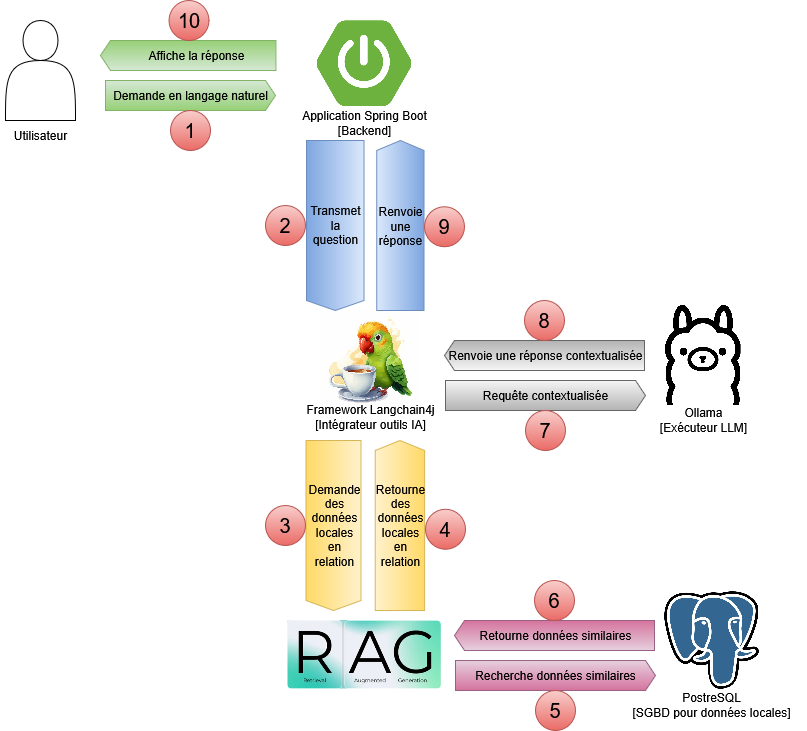
\includegraphics[width=1\textwidth]{illustration-graphique.drawio.png}
		\caption{Diagramme d'architecture}
		\label{fig:illustration-graphique}
	\end{figure}
	
	
	
	\section{Premier prototype}
	
	\subsection{Introduction}
	
	Pour atteindre cet objectif ambitieux, nous avons suivi une approche incrémentale. Dans un premier temps, un prototype fonctionnel a été réalisé afin de valider les fondements techniques du projet. Ce prototype est une application basée sur un agent intelligent exploitant une architecture RAG (Retrieval-Augmented Generation), capable de répondre aux questions de l’utilisateur à partir d’un document texte ou PDF fourni. Cette première version a permis de :
	\begin{itemize}
		\item comprendre le fonctionnement du framework LangChain4j ;
		\item tester l’intégration avec le LLM Ollama ;
		\item valider le concept de récupération de contexte à partir de documents externes.
	\end{itemize}
	
	Pour tester ce prototype, nous avons fourni un fichier PDF, son contenu est une lettre de recommandation pour une étudiante appelée Nour, on a ensuite envoyé une question à propos de cette étudiante à l'agent AI, en utilisant un contrôleur web :
	
	\begin{figure}[H]
		\centering
		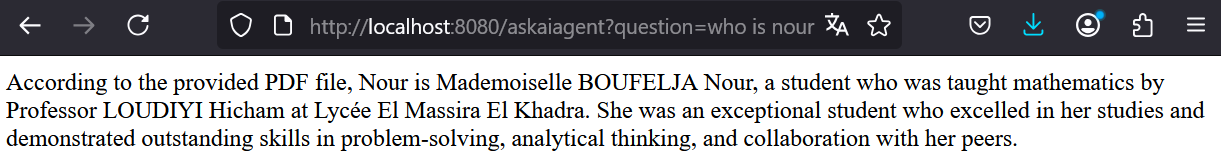
\includegraphics[width=\textwidth]{test-rag.png}
		\caption{Test du RAG}
		\label{fig:test-rag}
	\end{figure}
	
	
	
\end{document}}